%%%%%%%%%%%%%%%%%%%%%%%%%%%%%%%%%%%%%%%%%
% Focus Beamer Presentation
% LaTeX Template
% Version 1.0 (8/8/18)
%
% This template has been downloaded from:
% http://www.LaTeXTemplates.com
%
% Original author:
% Pasquale Africa (https://github.com/elauksap/focus-beamertheme) with modifications by 
% Vel (vel@LaTeXTemplates.com)
%
% Template license:
% GNU GPL v3.0 License
%
% Important note:
% The bibliography/references need to be compiled with bibtex.
%
%%%%%%%%%%%%%%%%%%%%%%%%%%%%%%%%%%%%%%%%%

\documentclass{beamer}

\usepackage{graphicx}
\usefonttheme{structuresmallcapsserif}
\usetheme{focus}

\vspace{-50pt}
\title{SDCEL}
\subtitle{Scalable Overlay Operations over DCEL Polygon Layers}

\author{
    Andres Calderon \textperiodcentered \ acald013@ucr.edu \\
    Amr Magdy \textperiodcentered \ amr@cs.ucr.edu \\ 
    Vassilis Tsotras \textperiodcentered \ tsotras@cs.ucr.edu
}

\institute{University of California, Riverside}

\begin{document}
    \begin{frame}
        \maketitle
    \end{frame}

    \begin{frame}{What is a DCEL?}
        \begin{minipage}{0.65\textwidth}
        \begin{itemize}
            \item Doubly Connected Edge List - DCEL.
            \item A spatial data structure collecting topological and geometric information for vertices, edges and faces contained by a surface in the plane.
            \item Widely use to support polygon triangulation and its applications (art gallery problem, robot motion planing, circuit board printing, etc).
        \end{itemize}
        \end{minipage}\hfill % maximize the horizontal separation
        \begin{minipage}{0.34\textwidth}
            \centering
            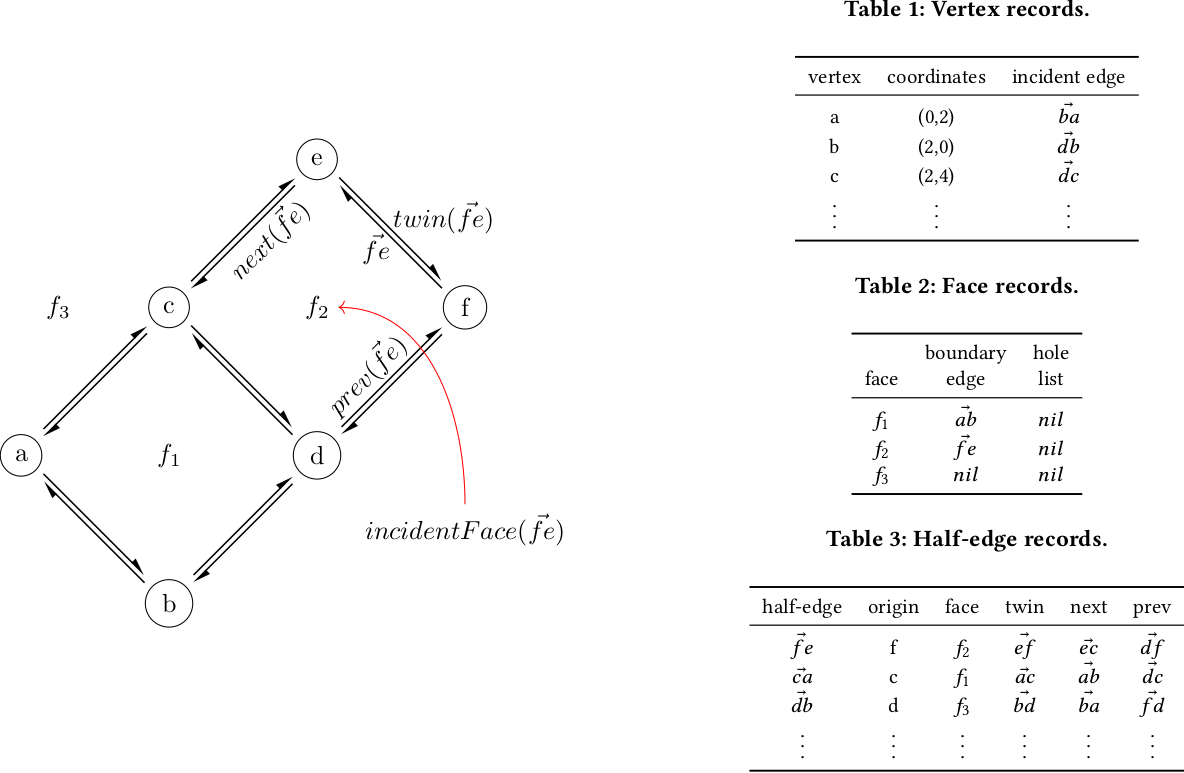
\includegraphics[width=\textwidth]{figures/dcel_example}
        \end{minipage}
    \end{frame}

    \begin{frame}{DCEL description}
        \begin{minipage}{0.49\textwidth}
            \centering
            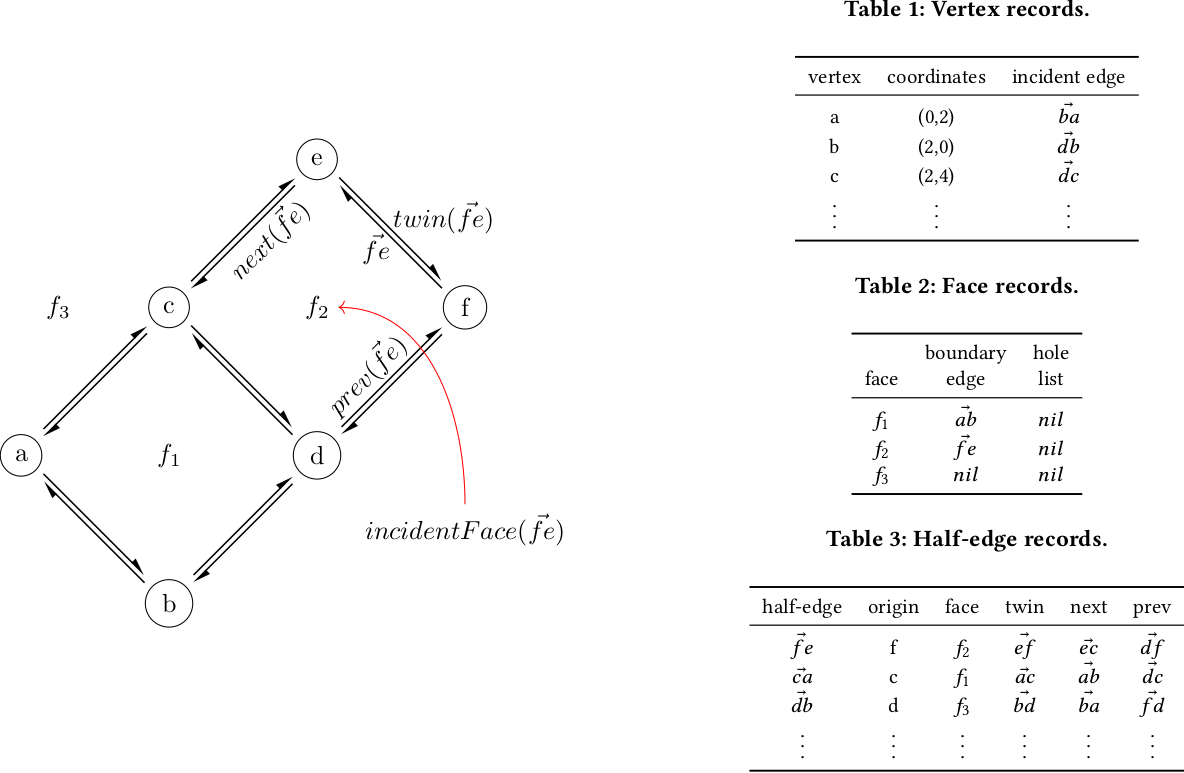
\includegraphics[width=0.9\textwidth]{figures/dcel_example}
        \end{minipage}\hfill % maximize the horizontal separation
        \begin{minipage}{0.49\textwidth}
            \centering
            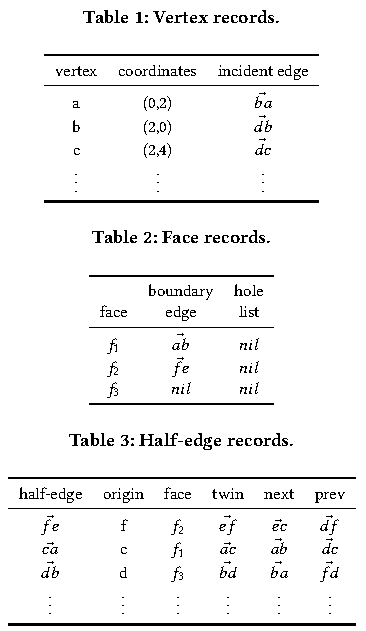
\includegraphics[width=0.7\textwidth]{figures/dcel_records}
        \end{minipage}
    \end{frame}

    \begin{frame}{Advantages, challenges and contributions}
        \begin{itemize}
            \item Very efficient for computation of \textit{overlay maps} and \textit{overlay operators}.
            \item Allows multiple operations over the same DCEL and chaining.
            \item Currently only sequential implementations.
            \item Unable to deal with large datasets (i.e. US Census tracks at national level).
            \item We propose a scalable and distributed approach to compute the overlay between two DCEL layers.
            \item It solve issues related to holes and large empty areas in addition to optimizations during the overlay computations.  
        \end{itemize}
        \vspace{0.25cm}

        \centering
        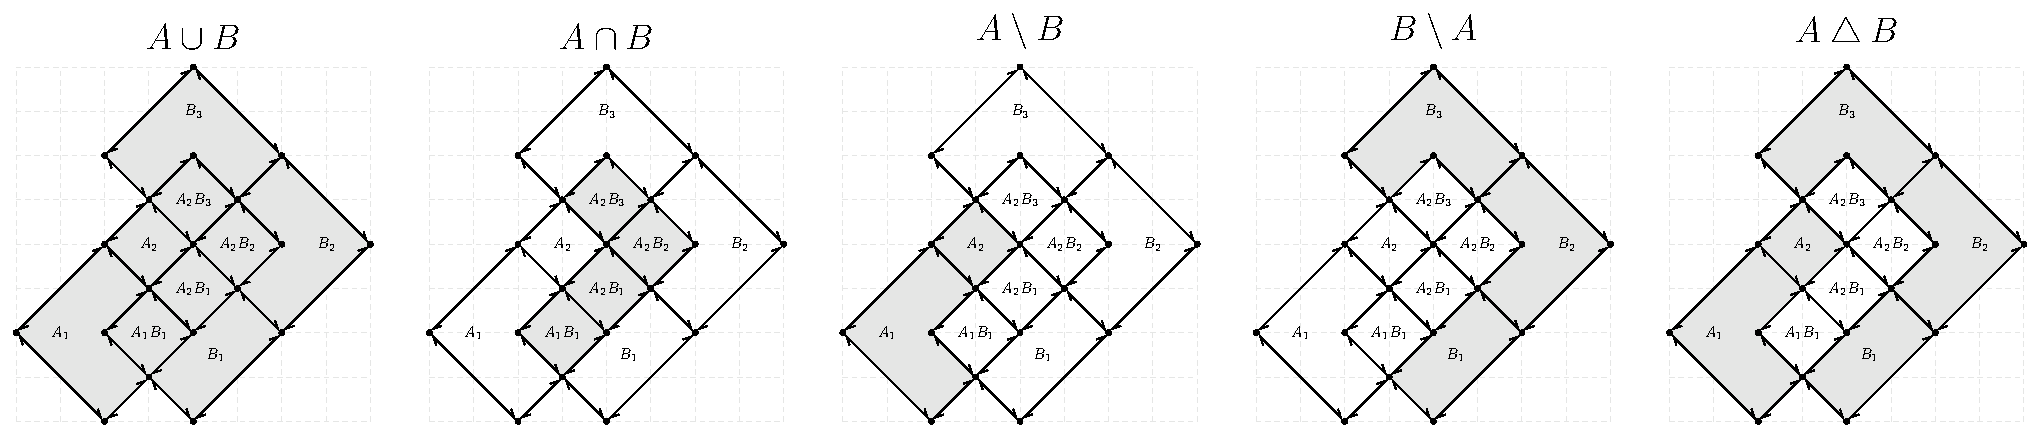
\includegraphics[width=0.9\textwidth]{figures/dcel_operators}        
    \end{frame}
    
    \begin{frame}{Sequential implementation}
        \centering
        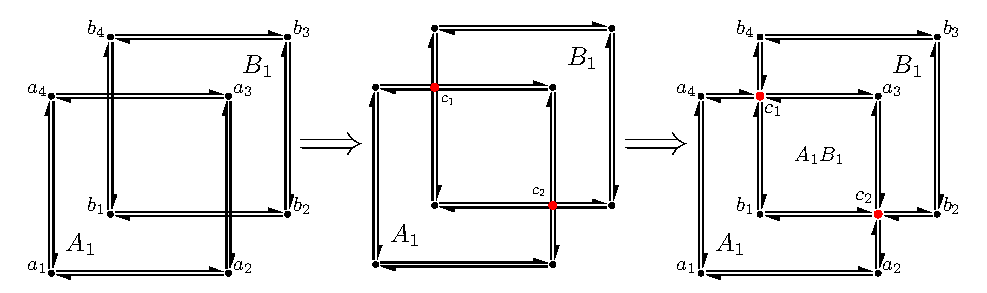
\includegraphics[width=\textwidth]{figures/dcel_seq}
    \end{frame}
    
    \begin{frame}{Partition strategy}
        \centering
        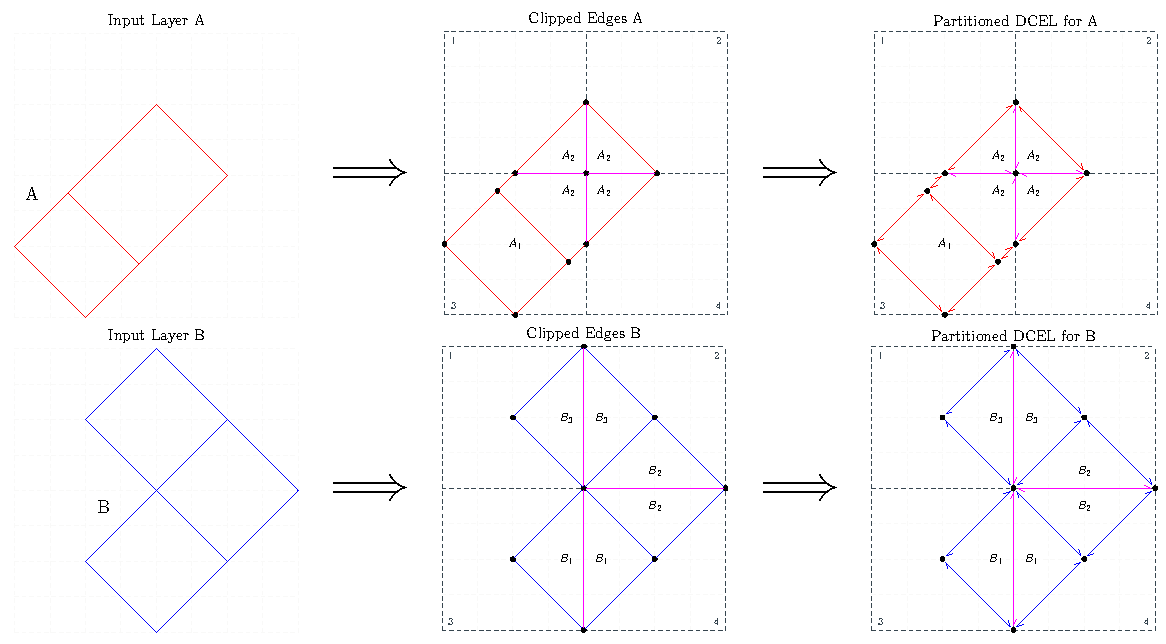
\includegraphics[width=0.8\textwidth]{figures/partition_strategy}
    \end{frame}

    \begin{frame}{Distributed DCEL construction}
        \centering
        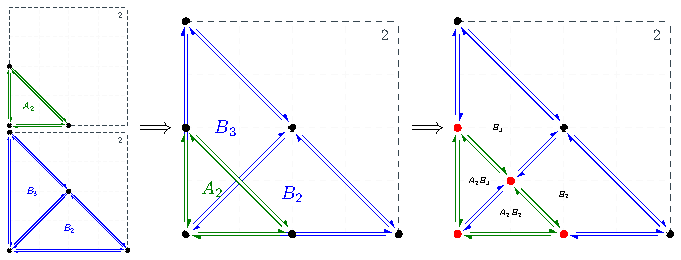
\includegraphics[width=0.55\textwidth]{figures/overlay_partition} \\
        \vspace{0.5cm}
        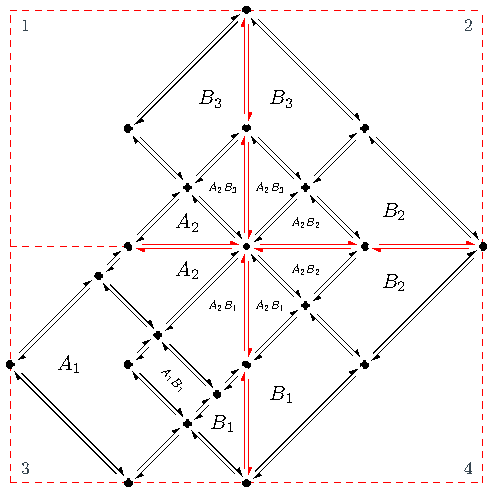
\includegraphics[width=0.35\textwidth]{figures/distributed_dcel}
    \end{frame}

    \begin{frame}{Labeling orphan cells and holes}
        \begin{minipage}{0.59\textwidth}
            \begin{itemize}
                \item The \textbf{orphan cell} problem.   
                \item When a cell is empty (it does not intersect or contain a \textit{regular edge}).
                \item A regular edge is one that is not part of a hole.
                \item The label for the cell (or a hole if it is present) is lost. Thus we do not know which face it belongs to.
                \item We provide algorithms to solve the issue.  
            \end{itemize}
        \end{minipage}\hfill % maximize the horizontal separation
        \begin{minipage}{0.4\textwidth}
            \centering
            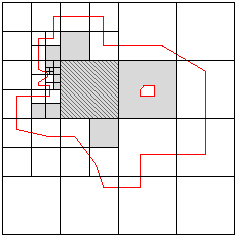
\includegraphics[width=\textwidth]{figures/holes1}
            \end{minipage}
    \end{frame}
    
    \begin{frame}{Labeling orphan cells and holes}
        \centering
        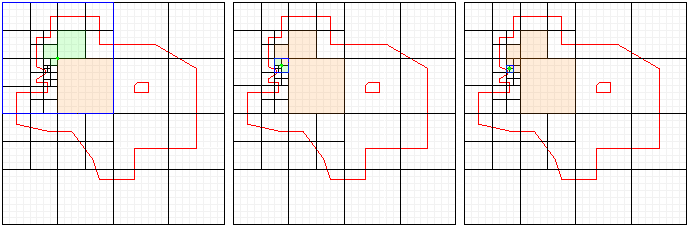
\includegraphics[width=\textwidth]{figures/holes2}
    \end{frame}

    \begin{frame}{Labeling orphan cells and holes}
        \begin{minipage}{0.49\textwidth}
            \centering
            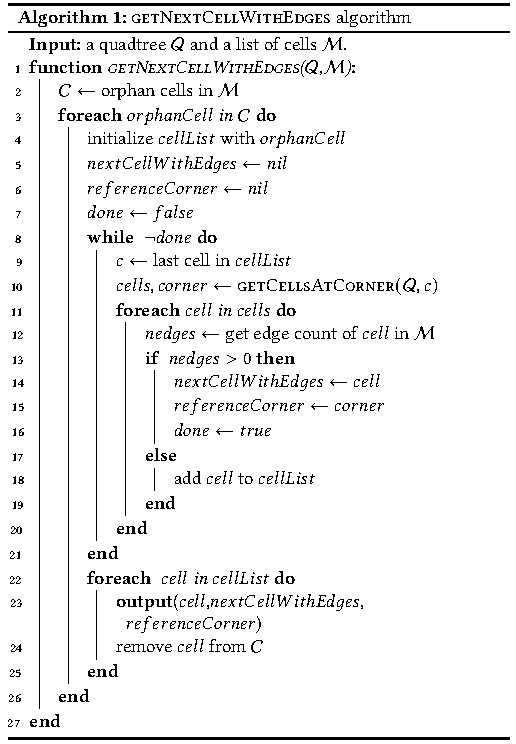
\includegraphics[width=0.8\textwidth]{figures/holes3}
        \end{minipage}\hfill % maximize the horizontal separation
        \begin{minipage}{0.49\textwidth}
            \centering
            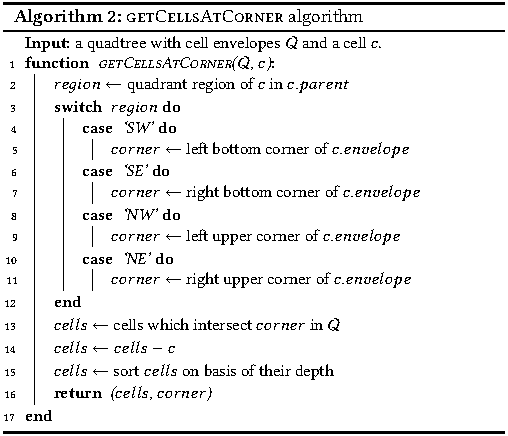
\includegraphics[width=0.8\textwidth]{figures/holes4}
        \end{minipage}
    \end{frame}
    
    \begin{frame}{Overlay evaluation}
        \begin{itemize}
            \item Answering global overlay queries...
            \begin{itemize}
                \item We query local DCEL's for particular overlay operators.
                \item It filters out at each worker.
                \item SDCEL collects back and reduce the final answer (remove artificial edges and concatenate splits).
            \end{itemize}
        \end{itemize}
        \vspace{0.5cm}

        \centering
        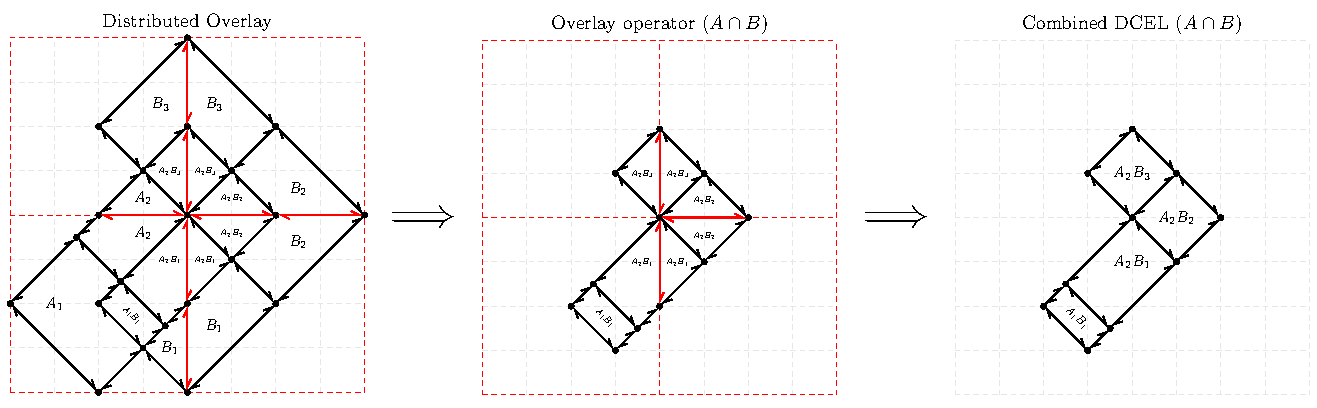
\includegraphics[width=\textwidth]{figures/overlay_operator}
    \end{frame}

    \begin{frame}{Overlay optimizations}
        \begin{itemize}
            \item Optimizations for faces expanding cells...
                \begin{itemize}
                    \item Naive approach send all faces to a master node.
                    \item We propose an intermediate reduce processing step.
                    \item The user provides a level in the quadtree structure and faces are evaluated at those intermediate reducers.
                    \item Another approach re-partitions the faces using its labels as the key.
                    \item It avoids the reduce phase but implies an additional shuffle.
                    \item However, SDCEL works with much smaller independent amounts of work.
                \end{itemize}
        \end{itemize}
    \end{frame}

    \begin{frame}{Overlay optimizations}
        \begin{itemize}
            \item Optimizing for unbalanced layers...
                \begin{itemize}
                    \item Finding intersections is the most critical part of the overlay computation.
                    \item However, in many cases one of the layer has much more half-edges than the other.
                    \item Sweep-line algorithms to detect intersections runs over all the edges.
                    \item We scan the larger dataset only for the x-intervals where there are half-edges for the smaller dataset.
                    \item It avoids unnecessary scanning where there are few edge (or even none) from one of the layers.
                \end{itemize}
        \end{itemize}
    \end{frame}
    
    \begin{frame}{Experimental evaluation}
        \begin{itemize}
            \item Datasets.
        \end{itemize}
        \vspace{1cm}
        \centering
        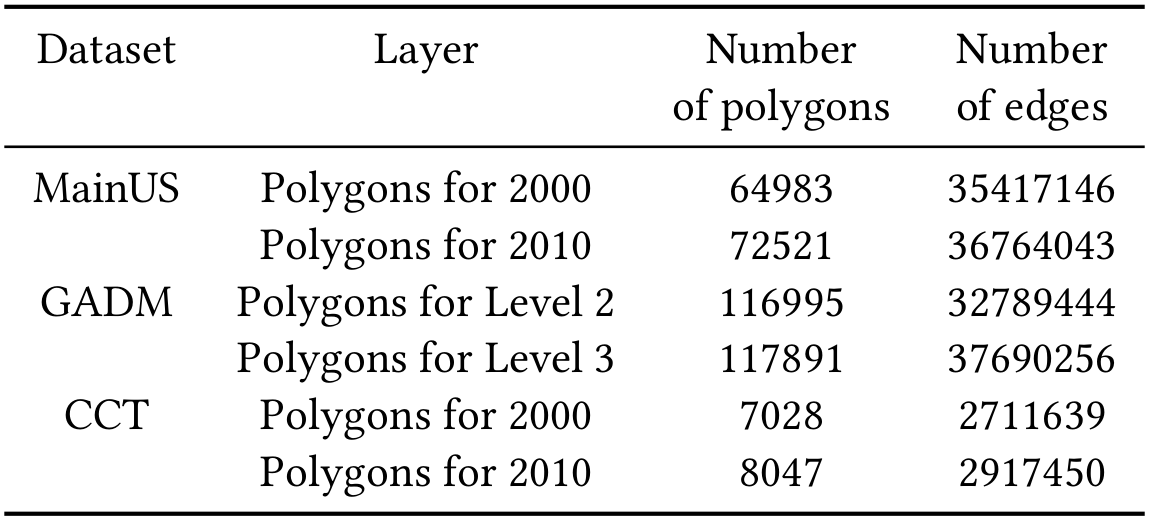
\includegraphics[width=0.75\textwidth]{figures/datasets}
    \end{frame}    
    
    \begin{frame}{Experimental evaluation}
        \begin{itemize}
            \item Evaluation of overlay methods.
        \end{itemize}
        \vspace{1cm}
        \centering
        \includegraphics[width=0.75\textwidth]{figures/overlay_tester}
    \end{frame}    

    \begin{frame}{Experimental evaluation}
        \begin{itemize}
            \item Unbalance layers optimization.
        \end{itemize}
        \vspace{1cm}
        \begin{minipage}{0.49\textwidth}
            \centering
            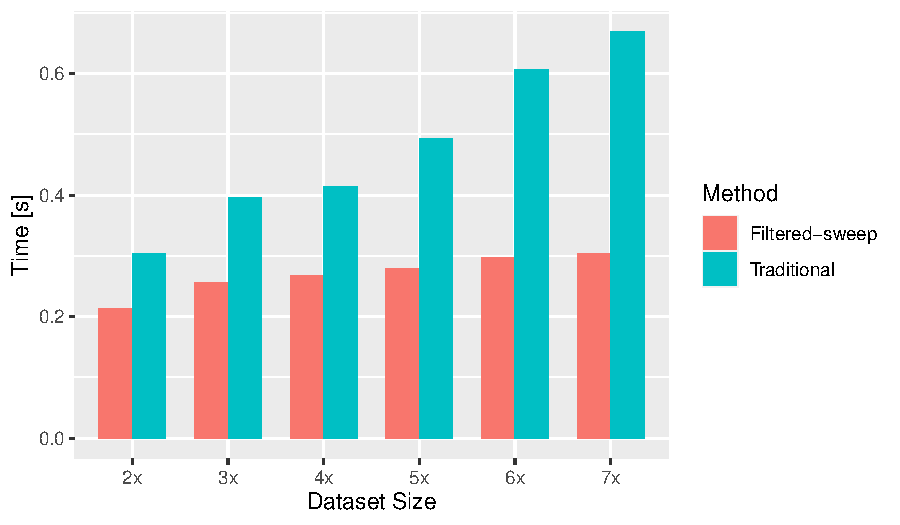
\includegraphics[width=\textwidth]{figures/unbalance1}
        \end{minipage}\hfill % maximize the horizontal separation
        \begin{minipage}{0.49\textwidth}
            \centering
            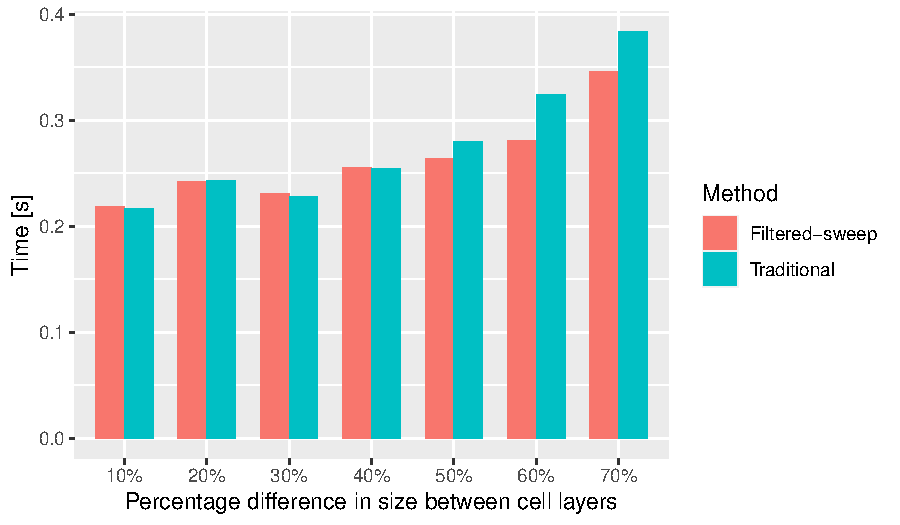
\includegraphics[width=\textwidth]{figures/unbalance2}
        \end{minipage}
    \end{frame}    

    \begin{frame}{Experimental evaluation}
        \begin{itemize}
            \item Performance varying number of cells (CCT dataset).
        \end{itemize}
        \vspace{1cm}
    
        \begin{minipage}{0.49\textwidth}
            \centering
            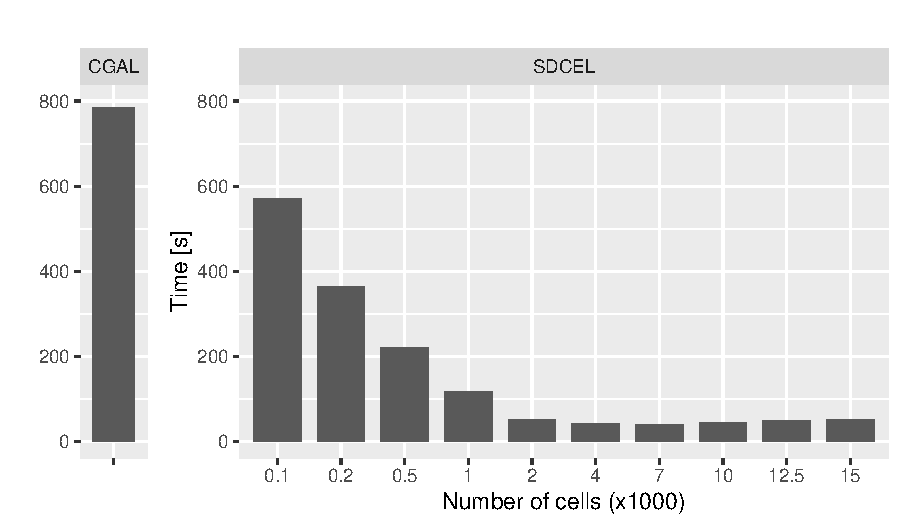
\includegraphics[width=\textwidth]{figures/ca}
        \end{minipage}\hfill % maximize the horizontal separation
        \begin{minipage}{0.49\textwidth}
            \centering
            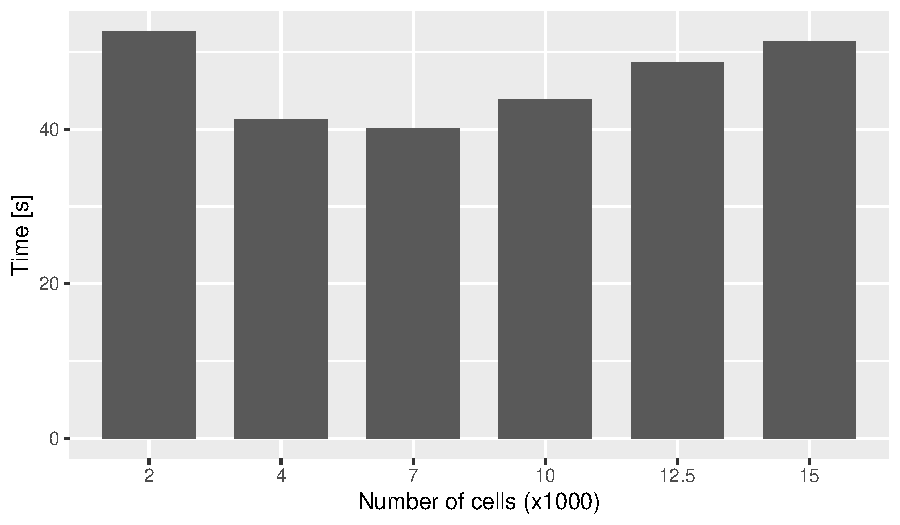
\includegraphics[width=\textwidth]{figures/ca_sample}
        \end{minipage}
    \end{frame}    

    \begin{frame}{Experimental evaluation}
        \begin{itemize}
            \item Performance with MainUS and GADM datasets.
        \end{itemize}
        \vspace{1cm}

        \begin{minipage}{0.49\textwidth}
            \centering
            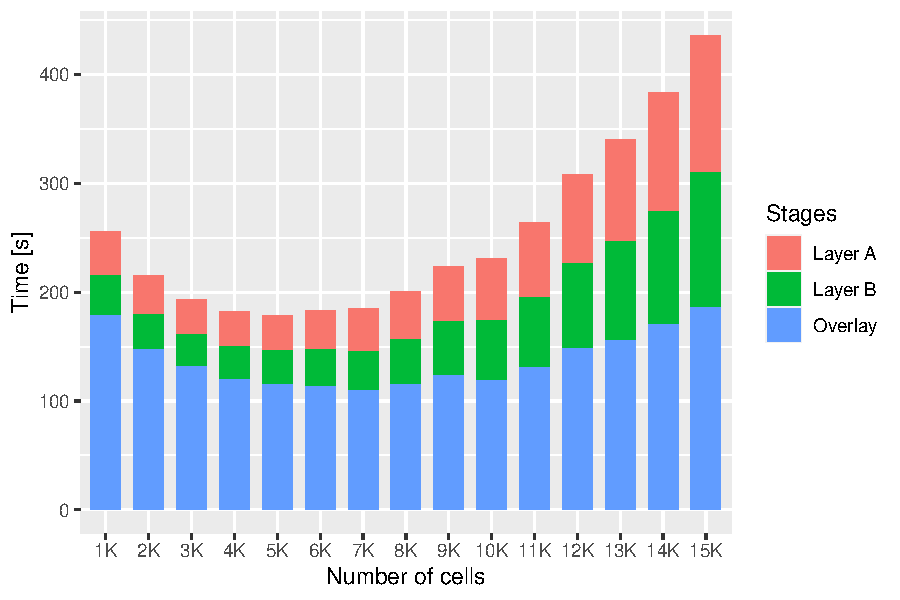
\includegraphics[width=\textwidth]{figures/mainus}
        \end{minipage}\hfill % maximize the horizontal separation
        \begin{minipage}{0.49\textwidth}
            \centering
            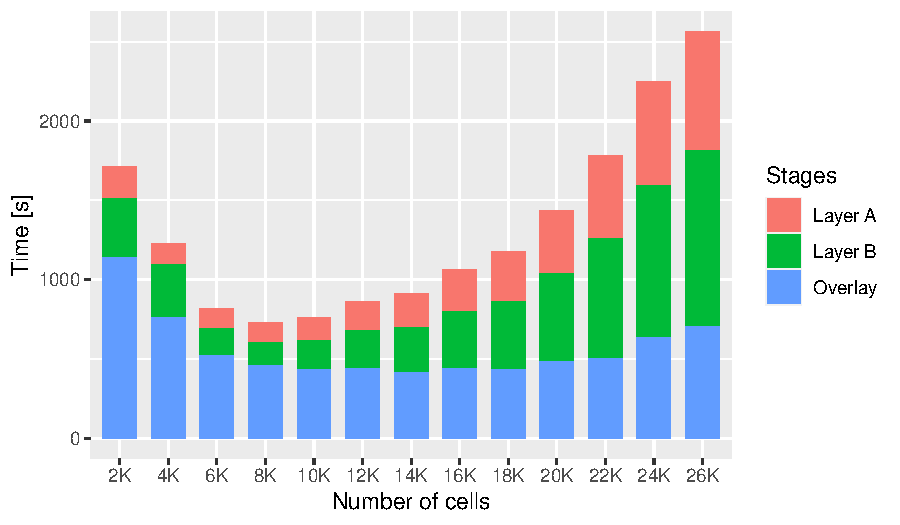
\includegraphics[width=\textwidth]{figures/gadm}
        \end{minipage}
    \end{frame}       
    
    \begin{frame}{Conclusions}
        \begin{itemize}
            \item We introduced SDCEL, a scalable approach to compute the overlay operation among two layers that represent polygons from a planar subdivision of a surface.
            \item We first presented a partition strategy which guarantee each partition has the needed data to work independently.
            \item We also proposed several optimization to improve performance and ensure correct results.
            \item Our experiments in real datasets show very good performance and it is able to compute overlays over very large layers in few minutes.
        \end{itemize}
    \end{frame}    

\end{document}
